%!TEX root = thesis.tex

%% ==============
\chapter{Baseline system} %TODO
\label{ch:Content1}
%% ==============

A system for symbol recognition was already written and is described in \cite{Kirsch}.


%% ===========================
\section{Section 1}
\label{ch:Content1:sec:Section1}
%% ===========================

\dots


%% ===========================
\section{Section 2}
\label{ch:Content1:sec:Section2}
%% ===========================

\dots


%% content.tex
%%

%% ==============
\chapter{Artificial Neural Nets}
\label{ch:Content2}
%% ==============

\Glspl{ANN} are models for classification that were inspired by the brain.
They consist of artificial neurons and have a lot of different subtypes like
Feed Forward Neural Nets.


%% ===========================
%!TEX root = thesis.tex
\section{Artificial neurons}\label{sec:artificial-neurons}
%% ===========================

Artificial neurons are inspired by biological neurons. Signals are send within 
the cell by charged particles, so called \textit{ions}. But before a biological
neuron sends a signal, a threshold charge has to be reached at the axon
hillock. This threshold charge is called \textit{action potential}. The action
potential can be reached by multiple factors, but the one I want to focus on
are charges send by other neurons. Depending on where the other axon terminals
are located and how long the distance to the axon hillock is, the signal contributes
more or less to reaching the action potential. After that, it simply sends a
signal.

\begin{figure}[ht]
    \centering
    \subfloat[Biological Neuron]{
        \includegraphics*[width=0.48\linewidth, keepaspectratio]{figures/biological-neuron.jpg} 
        \label{fig:biological-neuron}
    }%
    \subfloat[Artificial Neuron]{
        \resizebox{0.45\linewidth}{!}{\input{figures/artificial-neuron.tex}}
        \label{fig:artificial-neuron}
    }%
    \label{fig:artificial-and-biological-neuron}
    \caption{Both neurons receive weighted input, apply a function to that and give output}
\end{figure}

Artificial neurons are similar. They receive at least one input and give at
least one output. Those inputs might get weighted as well as the output.

The neurons apply a function to the sum of all weighted inputs. This function
is also called \textit{activation function}.

An artificial neuron using the unit step function (see \cref{f:unitstep}) is called
a \textit{perceptron}.


The artificial neuron sums all weighted inputs $x_i \cdot w_i$ up
             and applies its activation function $f$ to it.

%% ===========================
\section{Feedforward Neural Nets}
\label{ch:Content2:sec:Section2}
%% ===========================

Feedforward neural nets don't have loops.

\section{Activation functions}
\begin{figure}[ht]
    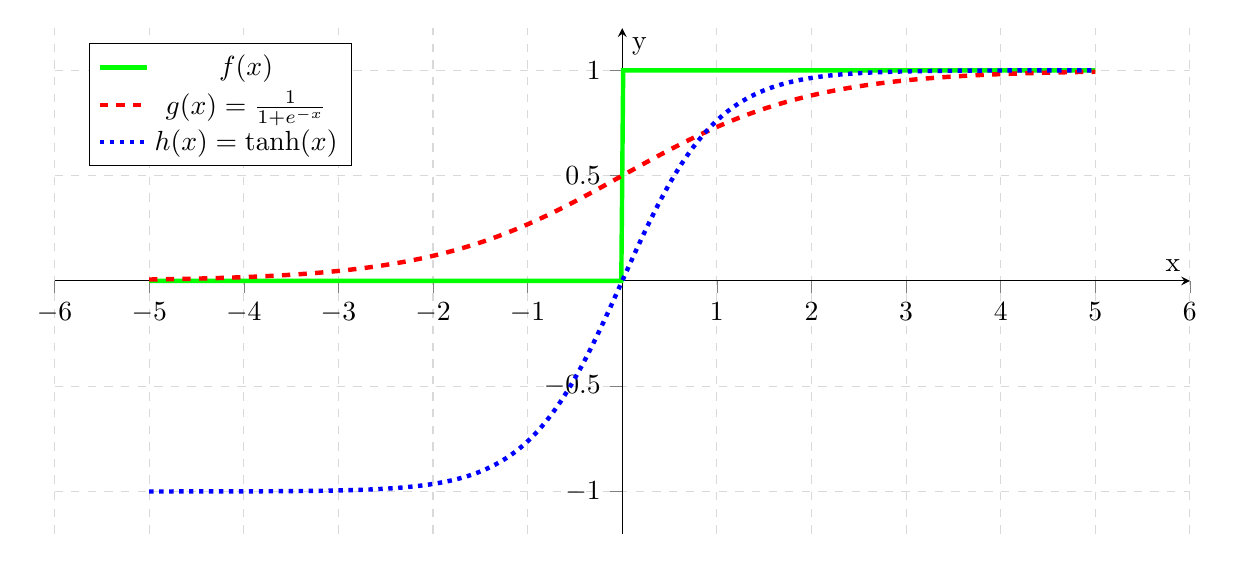
\begin{tikzpicture}[scale=1.0]
        \begin{axis}[
            legend pos=north west,
            axis x line=middle,
            axis y line=middle,
            grid = major,
            width=16cm,
            height=8cm,
            grid style={dashed, gray!30},
            xmin=-5,     % start the diagram at this x-coordinate
            xmax= 5,    % end   the diagram at this x-coordinate
            ymin=-1,     % start the diagram at this y-coordinate
            ymax= 1,   % end   the diagram at this y-coordinate
            %axis background/.style={fill=white},
            xlabel=x,
            ylabel=y,
            tick align=outside,
            enlargelimits=true]
          \addplot[domain=-5:5, green, ultra thick,samples=500] {x < 0 ? 0 : 1};
          \addplot[domain=-5:5, red, ultra thick,samples=500, dashed] {1/(1+exp(-x))};
          \addplot[domain=-5:5, blue, ultra thick,samples=500, dotted] {tanh(x)};
          \addlegendentry{$f(x)$} %TODO: \begin{cases} 0, & x < 0, \\ 1, & x \ge 0, \end{cases} (spacing)
          \addlegendentry{$g(x)=\frac{1}{1+e^{-x}}$}
          \addlegendentry{$h(x)=\tanh(x)$}
        \end{axis} 
    \end{tikzpicture}
    \caption{The unit step function $f$, the sigmoid function $g$ and the hyperbolic tangend $h$.}
    \label{fig:logistic-function}
\end{figure}

\subsection{Unit step function}\label{f:unitstep}


\subsection{Sigmoid function}\label{f:sigmoid}



\subsection{Hyperbolic tangent}\label{f:tanh}